\chapter{Technologies and Implementation}
\label{cha:tech}
The chapter covers the whole structure of the Python script used to both create the support model and also the simulator to measure the performance of each infecting strategy.

\section{Python}
\label{sec:python}
Everything is implemented through  a Python Program that allows to fetch the data, create the core structure of the network, compute functions, implement the seeding strategies and obviously run the simulations to measure the results and plot them to give graphic user friendly representations of the results.
A few support libraries are used for the above mentioned implementations, including:
\begin{itemize}
\item DyNetX to create the core network structure
\item MatplotLib to display a single simulation's result through a line chart (number of Infected nodes over time)
\item Math and Random to compute functions and generate random probability values
\end{itemize}

\subsection{DyNetx Library}
\label{sec:dynetx}
The Network is designed as a Temporal Directed Graph G. To do that DyNetX is used. It is a free open source Python Library that implements data structures to create and analyze temporal networks. The library is based on Networkx, and adds the temporal feature to all the data structures. This makes it extremely user friendly since it extends all common graphs concepts and methods to bring them to a temporal context. Some useful DyNetX methods include:
\begin{itemize}
\item Automatically build a dynamic graph from a text file
\item Compute Node Degree at a specific time or time window
\item Slice a Graph in time windows, or extract sub graphs at specific time or time window
\end{itemize}

\subsection{Network Nodes}
\label{sec:nodes}
Nodes are represented as Objects, with respective Id, Status and Cost as main attributes. Other attributes such as degree and neighbors are not needed as they can be easily computed dynamically and are not of common interest in all the proposed solutions, and are therefore computed and/or stored in memory only when needed. Id is fetched from the dataset while status and cost are initialized to Susceptible and zero. Status is then set to Infected for the selected Seed nodes, while cost is calculated for each node through the next mentioned loop.

\section{Script Structure}
\label{sec:script}
The script is coded to sequentially perform the following actions:
\begin{itemize}
\item Parse a dataset and build a Dynamic Directed Graph
\item Loop through each node to compute its cost to be selected in the initial Seed Set
\item Select a proposed strategy (selecting Pspread and total budget values)
\item Change the state of the Seed nodes to Infected
\item Run the simulation and display the run's result with an easy line chart to show the Influence Progression over time

\end{itemize} 
\hrule 
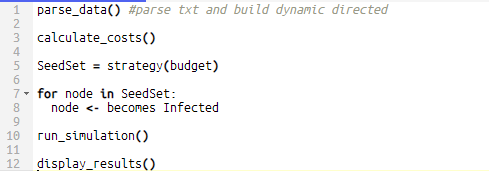
\includegraphics[]{script_structure}
\hrule

\begin{center}
    Figure 3.1: Pseudo code sum up for the entire script
\end{center}

\subsection{Simulation and Results Display}
\label{sec:run}
The simulation algorithm is implemented following the time order of the Network itself. Given the Seed Nodes as Infected and all the other ones as Susceptible, nodes interactions are scanned in ascending order. Whenever an interaction is recognized to be happening from an Infected node to a Susceptible one, the Susceptible node changes its state to Infected with fixed probability Pspread. At any time change information about the Influence progress is fed to the plot so that the final display can also better cover the Influence curve, to show the Infection progress very clearly throughout the time.
\\
\hrule 
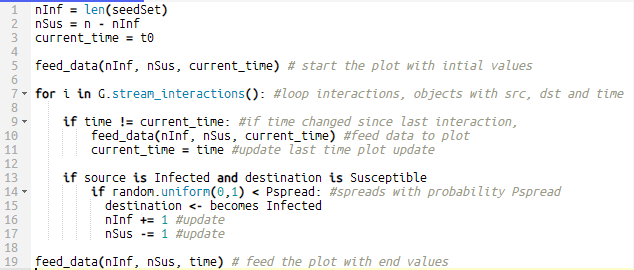
\includegraphics[]{code_simul}
\hrule

\begin{center}
    Figure 3.2: Pseudo Code for Simulation Run
\end{center}

The Single Simulation Plot allows the user to really see in detail how the curve of the Infection evolves throughout the time. This is interesting not only for the fact that it gives a visual representation of the result but also because it can underline the difference between different strategies and different network types. \\

\begin{center}
    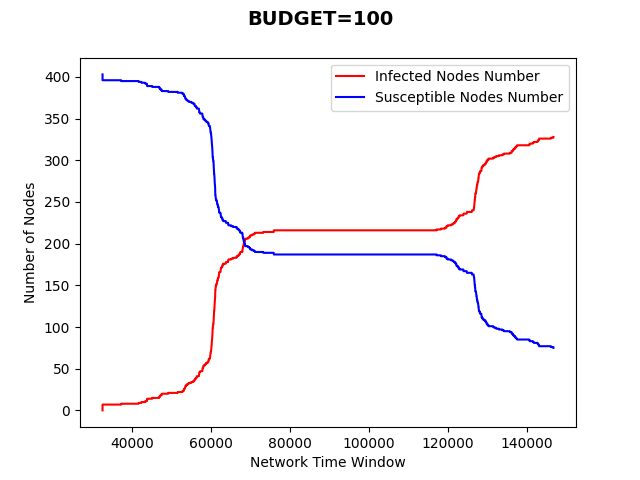
\includegraphics[scale=0.8]{line chart}\\
    Figure 3.3: Final Display of The Single Simulation Results
\end{center}

When working with temporal networks each interaction happens at a discrete time and so is everything that comes with it like nodes changing their state and network state update; this means that network structure and seed selection play a crucial role in determining the type of curve of infection. It can space anywhere between being a slow progressing curve or an early spiked curve. This allows strategies that aim at creating an early spike curve to maximize the time window where Infected users are actively interacting with the network, rather than "wasting" potential time and all the interactions that might occur in that window.\\


